\chapter{Diseño}
\label{sec:diseno}

%Es uno de los capítulos más importantes. Debe explicar claramente la solución propuesta justificando la aproximación adoptada. Este capítulo, según el caso, es aconsejable que defina claramente la arquitectura del sistema propuesto, identificando los roles o partes o actores del sistema. Pueden emplearse metodologías basadas en diagramas de clases, paquetes, diagramas secuenciales, diagramas de relación, etc.

%Si se ha diseñado una interfaz gráfica debe también describirse su estructura, dónde se mostrará la información, etc.

Este capítulo de diseño abarca una explicación de los bloques que se encuentran en la parte práctica del proyecto. Además del diseño, reflejado en un diagrama de bloques, que se ha seguido a la hora de implementar el prototipo de la \textit{blockchain}.\\

ARK \textit{deployer} \cite{deployer} da la posibilidad a cualquier usuario de crear una cadena de bloques independiente y funcional, que se puede personalizar de forma intuitiva. Dentro a del \textit{deployer} existen tres posibles configuraciones de la red (\textit{testnet}, \textit{devnet} y \textit{mainnet}). La red \textit{testnet} permite realizar cambios en una red local y privada, se puede personalizar entre otras cosas la moneda, la interfaz o en nuestro caso el algoritmo de firma. La red \textit{devnet} es una red de desarrollo no privada sino que cualquier persona puede acceder a ella para realizar cambios, la moneda que se utiliza se llama DARK. Y finalmente, la red \textit{mainnet} puedes personalizar la interfaz. \\

El \textit{core} gestiona todo lo referente a la creación de bloques y al almacenamiento de las transacciones en el mismo. Por tanto será la parte en la que se introduzca el algoritmo de firma y verificación la firma de los bloques. A causa de modularidad de las funciones del \textit{core}, se puede modificar una parte código y ajustarla a las necesiadades del usuario, sin tocar otras funciones. El \textit{core} como su propio nombre indica es el centro del prototipo, puesto que será el que interactúe con la base de datos, con la aplicación Wallet y con el \textit{explorer} de ARK. Tratará con la base datos para almacenar la información actualizada de los bloques. Con el Wallet para admitir las nuevas transacciones y guardalas en un bloque. Y en último lugar, con el explorer para mostrar cualquier tipo de información.\\

\newpage
La base datos se encarga de almacenar y servir datos de las transacciones dentro de un nodo\cite{BD-ARK}. Algunos datos que recoge son el usuario que realiza la transacción, el bloque en el que se almacena o la cantidad enviada en la transacción.\\

La aplicación Wallet de ARK \cite{wallet} es un monedero de criptomonedas contruida para proporcionar la realización de transacciones y firma de mensajes de forma segura, puesto que nadie excepto el usuario podrá acceder a las claves privadas del monedero. Una ventaja de esta aplicación  es que se conecta con la \textit{blockchain} de forma instantánea, manteniendo siempre la \textit{blockchain} actualizada. Se puede descargar para ordenadores, versión Desktop Wallet, está disponible para los principales sistemas operativos como MacOS, Windows y Linux. También se encuentra una versión para móviles, Mobile Wallet, compatible con \textit{smartphones} de \acrshort{ios} o android.\\

El \textit{explorer} de ARK \cite{explorer} es una interfaz muy intuitiva que recoge toda la información referente a las transacción. Los usuarios pueden acceder al estado de una transacción, realizada con el Wallet de ARK, para comprobar si ha llegado a su destino o si la han recibido. Pero no solo los usuarios que realizan dichas transacciones pueden visualizar el estado, sino que cualquier persona tiene acceso a este buscador de bloques, obtiendo cualquier información de la \textit{blockchain}. Las principales acciones que se pueden realizar en el \textit{explorer} de ARK son la búsqueda de un bloque creado, ver cada transacción realizada a una dirección, listar las direcciones de los monederos de ARK o incluso la instantánea del estado de la red.\\

El prototipo de instalación de la \textit{blockchain} modificada que se ha realizado en el docker, recoge todos bloques anteriormente citados, estos son el \textit{deployer}, el \textit{core}, la base de datos, la aplicación Wallet y el \textit{explorer} de ARK.\\

La figura \ref{fig:diag-bloques-1} muestra un diagrama con los bloques con el diseño general que se ha implementado. En el docker se incluye el \textit{deployer} que instala el \textit{core} de la cadena de bloques. Además, se encuentra la base de datos \texttt{postgresql}, que estará en interacción con el \textit{core}.\\

Por otra parte, fuera del docker, se encuentra el \textit{explorer} y la aplicación Desktop Wallet. El \textit{explorer} estará conectado al \textit{core} mediante el puerto API $4200$, al \textit{explorer} se podrá acceder mediante un navegador con la dirección \mbox{\texttt{http://NODE\_GENESIS:4200}}. Sin embargo, para acceder a la aplicación Desktop Wallet será necesario descargarla, veáse apéndice manual de usuario \ref{sec:manual-wallet}, dicha apliación se conectará con el \textit{core} mediante el puerto API $4103$.\\

%Los nombres de la bases de datos se pueden ver con el comando psql -l, y podemos ver que hay una para cada red, a nosotros no interesa core_bridgechain_testnet. Para visualizar las tablas poner el comando psql -U deployer - d core_bridgechain_testnet.

\begin{figure}[H]
	\centering
	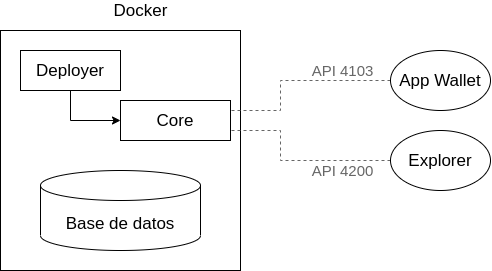
\includegraphics[width=0.8\textwidth]{figuras/diagrama_bloquesARK.png}
	\caption{Diagrama de bloques para el prototipo}
	\label{fig:diag-bloques-1}
\end{figure}

No hay una única configuración de los bloques. A modo de ejemplo se incluyen dos configuraciones diferentes. La primera, en la figura \ref{fig:diag-bloques-2}, muestra que no es necesario que la aplicación Wallet y el \textit{explorer} de ARK se encuentren en una misma máquina que el docker, es decir, que pueden alojarse en diferentes máquinas distribuidas y mediante una conexión por la red podrían comunicarse.\\ 

\begin{figure}[H]
	\centering
	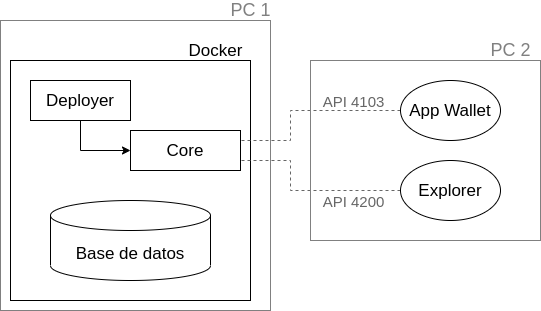
\includegraphics[width=0.8\textwidth]{figuras/diagrama_bloquesARK2.png}
	\caption{Diagrama de bloques. Ejemplo de configuración 1}
	\label{fig:diag-bloques-2}
\end{figure}

La segunda configuración, en la figura \ref{fig:diag-bloques-3}, muestra que tampoco tienen por qué, la aplicación Wallet y el \textit{explorer}, establecerse en la misma máquina. Dicha aplicación wallet se encuentra instalada en un \textit{smartphone}, puesto que dicha aplicación es compatible con dispositivos cuyo sistema operativo sea android o \acrshort{ios}.\\

\begin{figure}[H]
	\centering
	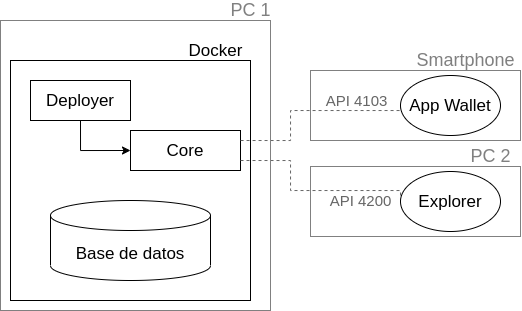
\includegraphics[width=0.8\textwidth]{figuras/diagrama_bloquesARK3.png}
	\caption{Diagrama de bloques. Ejemplo de configuración 2}
	\label{fig:diag-bloques-3}
\end{figure}


Finalmente, la estructura del algoritmo viene dada por un fichero escrito en python, denominado \texttt{uov.py}, donde se encuentran las funciones que se explicarán en detalle en el capítulo \ref{sec:implementacion}. Para continuar con la idea de modularidad de la arquitectura de ARK, la integración del algoritmo en la \textit{blockchain} se ha hecho en un fichero independiente. Esto es desde el archivo original donde se encuentran las funciones de firma y verificación de los bloques se creará un proceso que llame a las distintas funciones del algoritmo UOV.\\

El fichero \texttt{uov.py} incorpora main con un ejemplo de uso del algoritmo independientemente de la \textit{blockchain}. Dicho fichero se encuentra alojado en el \textit{core} de la cadena de bloques para utilizarlo en el algoritmo de firma y verificación.\\